
On donne l'algorithme suivant.
\parbox{0.28\linewidth}{
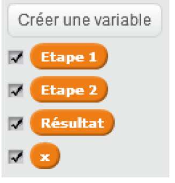
\includegraphics[scale=1]{NF-42.png} 
}
\parbox{0.48\linewidth}{
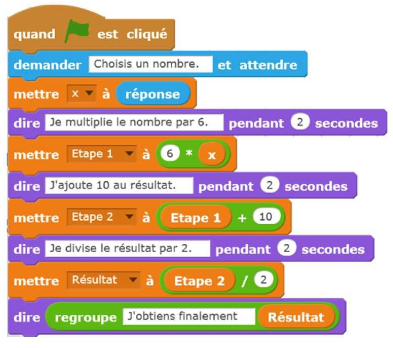
\includegraphics[scale=1]{NF-43.png}
}
\medskip

\begin{enumerate}
\item Si $a$ est le nombre choisi, déterminer l'image de $a$ par cet algorithme. On note $f(a)$ cette image.
\item Calculer $f\left(\frac{5}{6}\right)$.
\item Est-il possible que l'image de $a$ par cet algorithme soit égale à $a$ ? Justifier
\end{enumerate}